\chapter{M�todos}
\label{metodosec}

Este cap�tulo descreve todos os procedimentos de projeto e testes, dentre outros, empregados visando a obten��o do resultado final deste trabalho. Os procedimentos aqui empregados s�o embasados na teoria apresentada no cap�tulo \ref{EmbasamentoTeorico}. Cabe salientar que, embora este seja um projeto de integra��o entre \textit{mec�nica}, \textit{hardware} e \textit{software}, os esfor�os de desenvolvimento foram concentrados na �rea de desenvolvimento de \textit{softwares}, desde o servidor web e o algoritmo de controle implementados em Node.js, at� a aplica��o de usu�rio, escrita em diversas linguagens, de programa��o ou n�o --- a exemplo de HTML e CSS. A figura \ref{blocos} apresenta uma vis�o geral do sistema, que compreende parte mec�nica, \textit{hardware} e \textit{software}.

\begin{figure}[H]
	\centering
	\includegraphics[scale=0.40]{./Resources/diag_geral.png}
	\captionsetup{justification=centering}
	\caption[Diagrama em blocos do projeto]{Diagrama em blocos do projeto}
	\label{blocos}
\end{figure}

%%%%%%%%%%%%%%%%%%%%%%%%%%%%%%%%%%%%%%%%%%%%%%%%%%%%%%%%%%%%%%%%%%%

\section{Estrutura mec�nica}
\label{estmec}
Para o projeto da parte mec�nica, em primeiro lugar foi concebida uma configura��o de sistema baseada tanto na literatura dispon�vel quanto em projetos de sistemas comerciais de produ��o de cerveja: um sistema de duas panelas an�logas � MT e ao BK, sendo que durante o processo de cozimento do mosto, o BK pudesse ser utilizado como HLT. Para atender a esta especifica��o, fez-se necess�rio o projeto de um sistema de recircula��o entre as duas panelas. Obserava-se que esta proposta representa um h�brido entre o sistema de 3 panelas tradicional - que consiste de uma panela para mostura��o, uma para lavagem dos gr�os, ou \textit{sparging}, e uma para fervura; e o sistema popularizado pela Braumeister, composto de 1 panela, com recircula��o. Esta abordagem permitiu a economia financeira e simplifica��o mec�nica do sistema de tr�s panelas com o benef�cio do \textit{sparging} inexistente no sistema de uma panela.

\subsection{Funcionamento da estrutura}

Na figura \ref{esboco} � apresentada uma representa��o esquem�tica da parte funcional.

\begin{figure}[H]
	\centering
	\includegraphics[scale=0.55]{./Resources/esb_mec.jpg}
	\captionsetup{justification=centering}
	\caption[Representa��o esquem�tica da estrutura mec�nica]{Representa��o esquem�tica da estrutura mec�nica}
	\label{esboco}
\end{figure}

Na panela superior ou MT, rotulada como \textit{Mostura}, os gr�os s�o adicionados ap�s o aquecimento inicial da �gua:

\begin{itemize}
	\item A v�lvula 1 � uma v�lvula manual do tipo esfera, com passagem plena. Durante a opera��o do equipamento ela deve ficar sempre aberta, portanto seu uso � realizado somente em caso de emerg�ncias.
	\item Ap�s a adi��o dos gr�os, a bomba 3 � ligada para que o l�quido da panela seja recirculado. As v�lvulas de reten��o 11 e 12 n�o permitem que o l�quido passe por elas, portanto h� somente um caminho poss�vel para este, que � ascender pela tubula��o at� entrar novamente na MT. Note-se que n�o h� v�lvula automatizada na sa�da da MT, uma vez que o mosto fica em recircula��o constante ao longo do processo de cozimento.
	\item Ap�s a mostura a bomba 3 � desligada e a v�lvula solen�ide 2 � aberta, escoando o l�quido para a panela de fervura BK. Simult�neamente, a v�lvula solen�ide 7 e a bomba 8 s�o ativadas, fazendo com que a �gua de lavagem presente na BK/HLT flua pela tubula��o at� a MT, iniciando o processo de \textit{sparging}. Durante um tempo predefinido, o mosto e a �gua de lavagem recirculam pelas duas panelas e se misturam.
	\item Durante a fervura, as v�lvulas 2 e 7 s�o fechadas. Neste per�odo, os gr�os drenados que est�o na MT devem ser retirados manualmente, j� que ela ser� usada posteriormente para armazenamento da �gua de esfriamento do mosto --- �gua usada para limpeza do sistema e que reduz a produ��o de efluentes do mesmo.
	\item Ap�s a fervura, as v�lvulas solen�ides 7 e 10 s�o ativadas, permitindo o escoamento do l�quido para o trocador de calor. Simult�neamente a v�lvula solen�ide 13 � aberta e �gua fria circula em contra-fluxo para resfriar o mosto. Esta �gua sai quente do trocador de calor e passa pela v�lvula de reten��o 12, preenchendo a parte superior da tubula��o e sendo armazenada na MT para posterior limpeza do sistema.
	\item O mosto que sai resfriado do \textit{chiller} cai no balde de fermenta��o. Neste processo o l�quido entra em contato com o ar, o que � n�o somente desej�vel como essencial para o sucesso da fermenta��o, portanto esta � a �ltima parte automatizada que tem rela��o com a cerveja. Uma solu��o futura e que permite automa��o desta transi��o � o uso de um aerador em conjunto com um tanque de fermenta��o selado.
	\item Por fim, a �gua armazenada na MT � aquecida e recirculada pelo sistema, promovendo uma limpeza preliminar deste.
\end{itemize}

Para o bom funcionamento do sistema proposto, algumas condi��es devem ser atendidas:

\begin{itemize}
	\item Se o volume total de l�quido nas duas panelas ao final da mostura exceder o volume da BK, ela transbordar�. Por este motivo � importante que exista um sistema de detec��o de transbordo. Ainda assim, deve-se requisitar que o usu�rio do sistema calcule corretamente as propor��es da receita, pois mesmo que seja aplicado um sistema autom�tico anti-transbordo, ocorrer� perda de insumos devido ao ac�mulo de mosto inutiliz�vel na MT em caso de erro.
	\item S�o necess�rios filtros de material particulado na sa�da das panelas para o bom funcionamento das v�lvulas e bombas \cite{danfoss_solenoid}.
	\item Os dispositivos mec�nicos (v�lvulas, bombas, tubula��o, dentre outros) e eletr�nicos (sensores e atuadores) em contato com o sistema mec�nico devem ser apropriados �s altas temperaturas impostas pela natureza do processo \cite{danfoss_solenoid, jefferson_solenoid}.
	\item As panelas, tendo como refer�ncia seu fundo, n�o devem ser alinhadas conc�ntricas, j� que isto torna a adi��o de l�pulos e o processo de manuten��o do equipamento desajeitados.
	\item A automa��o da t�cnica de \textit{whirlpool} n�o � contemplada nesta configura��o de sistema. Se o usu�rio a considera necess�ria, ele deve se encarregar de execut�-la manualmente.
	\item A �nica v�lvula com press�o suficiente para ser servo-operada � a 13, assumindo-se que a press�o incidente sobre ela seja maior do que 0,5bar, portanto as outras devem ser de opera��o direta \cite{danfoss_solenoid, jefferson_solenoid}.
	\item A limpeza automatizada, ou CIP, n�o � contemplada em sua totalidade nesta configura��o do sistema, devido � alta complexidade \cite{cip_pres}, conforme indica a figura \ref{cip_system}, e ao custo de implementa��o proibitivo para o presente trabalho. N�o obstante, � recomendado ao usu�rio do sistema que fa�a a limpeza do mesmo t�o r�pido quanto poss�vel ap�s o final da produ��o.
\end{itemize}

\begin{figure}[H]
	\centering
	\includegraphics[scale=0.55]{./Resources/cip_example.jpg}
	\captionsetup{justification=centering}
	\caption[Sistema CIP b�sico]{Sistema CIP b�sico. \\Fonte: ROSE e MONTGOMERY (2010)}
	\label{cip_system}
\end{figure}

\subsection{Dimensionamento da parte funcional} 

Com a filosofia de opera��o do sistema mec�nico definida, foi poss�vel realizar o dimensionamento deste sistema. A primeira considera��o a ser feita � que os materiais e m�todos aqui empregados n�o seguem nenhuma norma que permita o uso deste equipamento para fabrica��o de cerveja visando sua comercializa��o --- tal escolha foi feita em fun��o do alto custo de um sistema completamente dentro das normas e tamb�m pelo fato de este ser um trabalho cujo foco � a automa��o e o acesso remoto do sistema, e n�o a comercializa��o de cerveja.

N�o obstante, o material da tubula��o escolhido foi o a�o inoxid�vel AISI304. J� que o volume de l�quido a ser trabalhado � pequeno, menor do que 40 litros, e a press�o de trabalho n�o � maior do que a press�o das bombas escolhidas posteriormente, foi decidido o uso de tubula��o de di�metro de 1/2" (21,34mm de di�metro externo) e espessura da parede no padr�o Schedule 40 (2,77mm de espessura). Embora esta espessura seja superdimensionada para a presente aplica��o, o mec�nico respons�vel pela montagem do sistema a requisitou para que fosse poss�vel fazer rosca sem danificar a integridade dos tubos. As conex�es, seguindo a escolha dos tubos, tamb�m foram de a�o inoxid�vel de 1/2".

As liga��es entre tubos, conex�es e outros componentes do sistema s�o liga��es rosqueadas. Este � um meio de liga��o antigo, por�m de baixo custo, f�cil execu��o e usualmente empregadas em tubula��es de di�metro nominal pequeno, menor do que 4" \cite{ifba}. Para veda��o foi escolhido o Teflon, uma vez que � um material de baixo custo e alta disponibilidade e o padr�o de rosca adotado neste projeto � o BSP, baseado na norma ISO. Cabe salientar que, embora as liga��es rosqueadas sejam permitidas sob certas circunst�ncias na pr�tica, elas s�o relegadas a instala��es de baixa responsabilidade \cite{ifba}.

As panelas foram escolhidas no material de alum�nio, em fun��o do custo proibitivo do a�o inoxid�vel. S�o caldeir�es padr�o utilizados no ramo de hotelaria e restaurantes e dispon�veis em v�rios volumes. As duas panelas utilizadas neste trabalho tem capacidade para 32 litros e di�metro do fundo de 36cm, portanto sua especifica��o no mercado � \textit{caldeir�o de alum�nio n. 36}. Tal volume, 60\% superior ao da produ��o m�xima aconselhada para este sistema, � necess�rio devido ao volume dos gr�os, � quantidade da �gua de lavagem e �s perdas por evapora��o que exigem uso de um volume de �gua inicial superior ao nominal.

O par�metro inicial escolhido para sele��o das v�lvulas solen�ide foi a temperatura m�xima de opera��o, cuja fonte de dados de opera��o � fornecida pelos fabricantes. Em seguida, foi escolhida uma veda��o adequada: os dois tipos mais comums de veda��o com suporte a temperatura de pelo menos 100\si{\degree}C s�o o EPDM e FKM (etileno-propileno-dieno e fluoreto de vinilideno, respectivamente) \cite{danfoss_solenoid}. Estes materiais possuem uma tabela de compatibilidade de fluidos cuja classifica��o pode ser satisfat�ria, boa, duvidosa, insatisfat�ria e desconhecida --- tanto para cerveja quanto para o mosto, ambas as veda��es s�o classificadas como satisfat�rias, embora para �gua a classifica��o do FKM seja somente boa \cite{epdm_fkm}. Por fim, um par�metro que foi verificado antes da escolha final das v�lvulas � a posi��o de opera��o, que varia conforme os modelos do fabricante \cite{danfoss_solenoid}. Com base nos par�metros supracitados, foi decidido usar:

\begin{itemize}
	\item V�lvula solen�ide 1/2" 12V pl�stico uso geral para �gua de resfriamento do trocador de calor.
	\item V�lvula solen�ide Danfoss 1/2" EV210BD 032U3620 para demais v�lvulas.
	\item Solen�ide Danfoss 15W 12VDC 042N7550 para acionamento das v�lvulas Danfoss.
\end{itemize}

Informa��es t�cnicas sobre a v�lvula EV210BD 032U3620 est�o no anexo \ref{Anexo3} e sobre a bobina 042N7550 no anexo \ref{Anexo4}.

As bombas de recircula��o foram escolhidas com base na temperatura de opera��o e grau aliment�cio. Posteriormente, tanto a vaz�o quanto a perda de carga do sistema foram estimadas para verificar se a bomba escolhida era adequada: o modelo Topsflo B08H-12-1006 tem capacidade m�xima de vaz�o de 10l/min e carga expressa em coluna de �gua de 6m. Como a capacidade m�xima do sistema � de 20l e idealmente a temperatura deve subir � taxa de 1\si{\degree}C/min, al�m de que a altura do sistema � menor do que 2m e as perdas de carga n�o decorrentes da gravidade foram consideradas desprez�veis para este caso, foi decidido que a bomba escolhida � adequada ao projeto. No \ref{Anexo5} encontra-se a folha de dados t�cnicos do dispositivo.

Quanto �s conex�es, a figura \ref{conexoes_rascunho} apresenta um diagrama conceitual do sistema, contendo as pe�as necess�rias para a montagem do mesmo:

\begin{figure}[H]
	\centering
	\includegraphics[scale=0.55]{./Resources/conexoes.jpg}
	\captionsetup{justification=centering}
	\caption[Diagrama conceitual das conex�es mec�nicas]{Diagrama conceitual das conex�es mec�nicas}
	\label{conexoes_rascunho}
\end{figure}

Na figura \ref{mt_cad} � apresentado um diagrama da MT constru�do no software FreeCAD, � qual est�o conectados o resistor de pot�ncia e um niple com veda��o. Tamb�m est�o presentes na figura a v�lvula esfera manual, um \textit{tee} f�mea, uma v�lvula Danfoss EV210B e tr�s niples de conex�o entre estes componentes. O modelo da v�lvula foi obtido a partir do website da Danfoss e importado, enquanto a modelagem dos outros componentes foi desenvolvida na plataforma FreeCAD. Na figura \ref{mt_cad_close} s�o apresentadas em detalhe as conex�es do resistor e do niple � panela e, por isto, a estrutura da mesma foi omitida. Os itens em amarelo s�o contra-porcas, em azul arruelas e, em vermelho an�is de veda��o (\textit{o-rings}).

\begin{figure}[H]
	\centering
	\begin{subfigure}{.46\textwidth}
		\centering
		\includegraphics[height=5cm]{./Resources/mecsys/mash-tun-top-color.pdf}
		\caption{Vista superior}
		\label{mt_cad:1}
	\end{subfigure}
	\begin{subfigure}{.46\textwidth}
		\centering
		\includegraphics[height=5cm]{./Resources/mecsys/mash-tun-bottom-color.pdf}
		\caption{Vista inferior}
		\label{mt_cad:2}
	\end{subfigure}
	\captionsetup{justification=centering}
	\caption[Diagrama da panela de mostura e conex�es]{Diagrama da panela de mostura e conex�es}
	\label{mt_cad}
\end{figure}

\begin{figure}[H]
	\centering
	\includegraphics[scale=0.35]{./Resources/mecsys/mash-tun-seal-color.pdf}
	\captionsetup{justification=centering}
	\caption[Detalhes da veda��o da panela de mostura]{Detalhes da veda��o da panela de mostura}
	\label{mt_cad_close}
\end{figure}

\newpage

\subsection{Estrutura met�lica de suporte}

Parte importante do projeto � o dimensionamento da estrutura met�lica de suporte �s panelas, j� que esta � respons�vel n�o somente pelo alojamento do sistema mec�nico como tamb�m pela facilidade de manuten��o. Para defini��o da posi��o das panelas, foram medidas primeiramente as suas alturas e da estrutura de adi��o de l�pulos (que ser� detalhada � parte na se��o \ref{hopbox}) e do \textit{chiller}. Na sequ�ncia, foi estimado um espa�o de manobra entre as duas panelas e uma altura m�nima do ch�o, com base na figura \ref{esboco}. Todas as medidas citadas est�o dispostas na tabela \ref{alturas}.

\begin{center}
	\begin{table}[H]
		\captionsetup{justification=centering}
		\caption[Dimens�es elementos mec�nicos relevantes para o projeto da altura da estrutura met�lica]{Dimens�es elementos mec�nicos relevantes para o projeto da altura da estrutura met�lica}
		\label{alturas}
		\begin{tabular}{ | M{10cm} | M{5cm} |}
			\hline
			\textbf{Descri��o} & \textbf{Altura (cm)} \\ \hline
			Panela BK & 30,0\\ \hline
			Panela MT & 30,0\\ \hline
			\textit{Chiller} & 30,0\\ \hline			
			Estrutura dos l�pulos aberta & 20,0\\ \hline
			V�o livre entre panelas & 20,0\\ \hline
			V�o do \textit{chiller} ao BK & 10,0\\ \hline
			Espa�o entre MT e topo & 10,0\\ \hline
		\end{tabular}
	\end{table}
\end{center}

Somando-se todos os valores da tabela \ref{alturas}, obteve-se que a estrutura met�lica deve ter 1,5m de altura. A largura deve ser de 36,5cm para acomodar as panelas com uma pequena folga e o comprimento escolhido � de 70cm, o que permite alinhar as panelas de maneira n�o conc�ntrica, conforme abordado na se��o \ref{estmec} --- este valor � suficiente, j� que o di�metro somado das duas panelas � de 72cm e � preciso que exista uma intersec��o para permitir o escoamento por gravidade da MT ao BK. Na figura \ref{estmec_cad} � apresentado o projeto da estrutura j� com as prateleiras para acomodar as panelas. Note-se que foram escolhidas cantoneiras de 2" x 1/8" para a constru��o deste equipamento.

\begin{figure}[H]
	\centering
	\includegraphics[scale=0.35]{./Resources/mecsys/estmec-freecad.pdf}
	\captionsetup{justification=centering}
	\caption[Projeto da estrutura met�lica]{Projeto da estrutura met�lica}
	\label{estmec_cad}
\end{figure}


%%%%%%%%%%%%%%%%%%%%%%%%%%%%%%%%%%%%%%%%%%%%%%%%%%%%%%%%%%%%%%%%%%%%%%%%%%

\section{Estrutura de adi��o de l�pulos}
\label{hopbox}
Devido � necessidade de adicionar l�pulos � receita em propor��es e tempos predefinidos, foi necess�rio o projeto de uma estrutura autom�tica de adi��o de l�pulos. Em fun��o das in�meras possibilidades de combina��es de l�pulos e temporiza��es, a escolha natural do projeto foi uma estrutura que permita esta flexibilidade --- uma caixa com oito compartimentos separados, que permite a adi��o sequencial destes insumos. Com base em um pacote de l�pulos em \textit{pellets} de 50g, estimou-se que seu volume � de $160cm^3$ e, sabendo-se que uma receita de 20l dificilmente utiliza uma quantidade maior do que 400g de l�pulos, a decis�o tomada foi a de que cada um dos 8 compartimentos deveria ter os $160cm^3$ necess�rios para acomodar 50g. Para confirmar que 400g � uma quantidade razo�vel, foi seguido o c�lculo de IBU de \cite{palmer}, detalhado no ap�ndice \ref{Ap�ndice C}.

Fixando a altura do compartimento em 10,0cm foram escolhidos valores de comprimento e largura de 16,0cm e 8,0cm respectivamente, assumindo inicialmente que as paredes das divis�rias tem espessura desprez�vel. A equa��o para volume de um prisma e a escolha das dimens�es s�o demonstradas em \ref{eq_hop_vini}:

\begin{subequations}
	\label{eq_hop_vini}
	\begin{align}
		V &= l\cdot w\cdot h = V_{50g}\cdot 8 \\
		&= l\cdot w\cdot 10 = 160\cdot 8 \nonumber \\
		l\cdot w\cdot &= 128, fixando \quad l = 16cm \quad \therefore \nonumber \\
		w &= 128/16 = 8cm \quad e \\
		w_{compartimento} &= l/8 = 16/8 = 2cm
	\end{align}
\end{subequations}

Posteriormente aos c�lculos de \ref{eq_hop_vini}, durante o projeto no software FreeCAD, observou-se que a assump��o de espessura desprez�vel � falsa e um retrabalho nas medidas do compartimento levou �s dimens�es externas finais de 18,0cm x 8,4cm x 10,0cm; as paredes externas tendo espessura de 3,0mm e as internas de 2,0mm. A figura \ref{caixa_cinza} esbo�a as dimens�es externas da caixa e a figura \ref{corpo_hopbox} apresenta o corpo da estrutura.

\begin{figure}[H]
	\centering
	\includegraphics[scale=0.35]{./Resources/estLup/caixa_lupulos(1).pdf}
	\captionsetup{justification=centering}
	\caption[Dimens�es da estrutura de adi��o de l�pulos]{Dimens�es da estrutura de adi��o de l�pulos}
	\label{caixa_cinza}
\end{figure}

\begin{figure}[H]
	\centering
	\begin{subfigure}{.46\textwidth}
		\centering
		\includegraphics[height=7.5cm]{./Resources/estLup/caixa_lupulos(2).pdf}
		\caption{Vista superior}
		\label{corpo_hopbox:1}
	\end{subfigure}
	\begin{subfigure}{.46\textwidth}
		\centering
		\includegraphics[height=7.5cm]{./Resources/estLup/caixa_lupulos(3).pdf}
		\caption{Vista axiom�trica}
		\label{corpo_hopbox:2}
	\end{subfigure}
	\captionsetup{justification=centering}
	\caption[Corpo da estrutura de adi��o de l�pulos]{Corpo da estrutura de adi��o de l�pulos}
	\label{corpo_hopbox}
\end{figure}

Foram projetadas duas portinholas: uma na face superior da caixa, para reabastecimento manual dos l�pulos, com uma al�a e fixada na caixa por dois pinos, de modo que a abertura desta tampa � um movimento de rota��o e; uma na face inferior para adi��o autom�tica, de correr, de modo que a abertura � um movimento de transla��o; ambas est�o ilustradas na figura \ref{tampas_hopbox}.

\begin{figure}[H]
	\centering
	\begin{subfigure}{.46\textwidth}
		\centering
		\includegraphics[height=7.5cm]{./Resources/estLup/caixa_lupulos(4).pdf}
		\caption{Tampa manual para reabastecimento}
		\label{tampas_hopbox:1}
	\end{subfigure}
	\begin{subfigure}{.46\textwidth}
		\centering
		\includegraphics[height=7.5cm]{./Resources/estLup/caixa_lupulos(5).pdf}
		\caption{Tampa para adi��o autom�tica dos l�pulos}
		\label{tampas_hopbox:2}
	\end{subfigure}
	\captionsetup{justification=centering}
	\caption[Tampas da estrutura de adi��o de l�pulos]{Tampas da estrutura de adi��o de l�pulos}
	\label{tampas_hopbox}
\end{figure}

Duas varetas de comprimento $l_1$ e $l_2$ s�o ligadas ao encaixa da tampa de correr, representada em azul na figura \ref{tampas_hopbox} (b), e a elas � acoplado um servo-motor cujo �ngulo de opera��o $\theta$ define a abertura --- ou deslocamento --- da tampa, definido por $d$. A figura \ref{varetas} esquematiza as liga��es.

\begin{figure}[H]
	\centering
	\includegraphics[scale=0.1]{./Resources/estLup/esquema-varetas.jpg}
	\captionsetup{justification=centering}
	\caption[Esquema de liga��o das varetas � tampa de correr]{Esquema de liga��o das varetas � tampa de correr}
	\label{varetas}
\end{figure}

Sendo o comprimento da tampa igual a $l_3$, a condi��o na equa��o \ref{eq_varetas} deve ser satisfeita para que a excurs�o m�xima de abertura da caixa possa ser atingida. � poss�vel demonstrar com o aux�lio da Lei dos Cossenos, em \ref{eq_cossenos} que $l_1 = l_2 = l$ para que a m�nima abertura da caixa possa ser atingida.

\begin{align}
	\label{eq_varetas}
	l_1 + l_2 \geq l_3
\end{align}

\begin{align}
	\label{eq_cossenos}
	&l_2^2 = d^2 + l_1^2 - 2dl_1\cdot cos(\theta) \\
	&se \quad \theta = 90\si{\degree} \rightarrow d = 0 \therefore \nonumber\\
	\label{res_cossenos}
	&l_2^2 = l_1^2 \rightarrow l_2 = l_1 = l
\end{align}

A taxa m�xima de deslocamento em fun��o do �ngulo do servo motor � expressa em \ref{eq_desl}:

\begin{align}
	\label{eq_desl}
	\frac{dl_3}{d\theta} = \frac{2l}{90\si{\degree}}
\end{align}

Entretanto, quanto maior o valor desta taxa, menor � a resolu��o de abertura da caixa, portanto obtem-se que o menor valor poss�vel de $l$, a partir da equa��o \ref{eq_varetas} � $l = l_3/2$. Assim sendo, a taxa de deslocamento calculada a partir da equa��o \ref{eq_desl} � de $2mm/\si{\degree}$.

Embora o valor te�rico de $\theta$ seja $90\si{\degree}$, na pr�tica, devido ao encaixe entre tampa e vareta n�o ser na extremidade, este valor � reduzido. Tal fato n�o deve ser negligenciado, uma vez que isto pode for�ar a opera��o do servo-motor ou quebrar alguma das pe�as do sistema. Sabe-se pelo projeto executado no FreeCAD que a dist�ncia da borda ao encaixe da tampa � de 2,3cm e portanto, com o aux�lio da Lei dos Cossenos, obt�m-se que $\theta_{max} = 82\si{\degree}$. Quanto ao valor m�nimo n�o h� preocupa��o, j� que a abertura da caixa ter� uma excurs�o reduzida em 2,3cm com rela��o ao seu comprimento. As varetas n�o foram calculadas novamente para corrigir esta excurs�o pois a redu��o foi considerada uma boa pr�tica, que evita que a tampa se desacople da caixa. A figura \ref{completa_hopbox} apresenta o esquema completo de constru��o da estrutura de adi��o de l�pulos.

\begin{figure}[H]
	\centering
	\includegraphics[scale=0.25]{./Resources/estLup/final.jpg}
	\captionsetup{justification=centering}
	\caption[Estrutura de adi��o de l�pulos]{Estrutura de adi��o de l�pulos}
	\label{completa_hopbox}
\end{figure}

\subsection{Controle do servo-motor}

Servomotor � um dispositivo de convers�o eletromec�nica que surgiu da necessidade de controle de posi��o angular de um motor de corrente cont�nua --- tanto � que um servomotor � um motor DC com controle e realimenta��o, ou seja, um dispositivo de malha fechada. Al�m da tens�o de alimenta��o, o servomotor recebe um sinal de controle proporcional � posi��o desejada do eixo e atua no motor DC at� que, atrav�s do ramo de realimenta��o, atinja-se a posi��o angular de entrada. A Figura \ref{servo_desmontado} apresenta um servomotor desmontado e a identifica��o de suas partes principais.

\begin{figure}[H]
	\centering
	\includegraphics[scale=0.50]{./Resources/servo/partes.png}
	\captionsetup{justification=centering}
	\caption[Servo-motor desmontado]{Servo-motor desmontado}
	\label{servo_desmontado}
\end{figure}

Observa-se que o circuito de controle � um circuito integrado, por�m n�o h� ampla documenta��o acerca de sua arquitetura interna; j� o potenci�mentro � o elemento sensor do conjunto, cujo objetivo � fornecer a posi��o angular do eixo atrav�s da varia��o de sua resist�ncia. O motor � a planta do sistema de controle, convertendo energia el�trica em rota��o do eixo. O conjunto de engrenagens � respons�vel por aumentar o torque do mesmo, com a diminui��o da velocidade de rota��o.

A caracteriza��o funcionamento do servomotor foi realizada em 4 partes: elabora��o do c�digo de controle para 8051; simula��o no software Proteus ISIS; ensaio para determinar os valores pr�ticos de opera��o do servomotor e; nova simula��o no software Proteus ISIS. O c�digo para AT89S52 --- compat�vel com 8051 --- � apresentado na caixa \ref{at_servo_code} do ap�ndice \ref{apendice_servo} e o diagrama esquem�tico do circuito de teste e simula��o na figura \ref{circuito_servo}. O uso do AT89S52 se deve ao fato de que o uso do PWM com a BBB ainda n�o estava desenvolvido neste ponto do projeto, por�m posteriormente a interface entre servo-motor e BBB foi realizada --- e os resultados est�o descritos na se��o \ref{aciona_results}.

\begin{figure}[H]
	\centering
	\includegraphics[scale=0.23]{./Resources/servo/diagrama_esquematico.png}
	\captionsetup{justification=centering}
	\caption[Circuito de caracteriza��o do servo-motor]{Circuito de caracteriza��o do servo-motor}
	\label{circuito_servo}
\end{figure}

Observa-se a necessidade de um buffer entre o microcontrolador AT89S52 e o servomotor, pois a corrente requisitada pelo pino de controle do servo � maior do que a corrente m�xima fornecida pelo \si{\micro}C. 

Os resultados da caracteriza��o do funcionamento do servo-motor est�o documentados no ap�ndice \ref{apendice_servo}.













%%%%%%%%%%%%%%%%%%%%%%%%%%%%%%%%%%%%%%%%%%%%%%%%%%%%%%%%%%%%%%%%%%%%%%%%%%

%\section{Configura��o da BeagleBone Black}
%BBB � uma placa de sistema embarcado desenvolvida para a comunidade de c�digo aberto (\textit{open-source}), iniciantes e quaisquer pessoas interessadas em um sistema equipado com um processador ARM Cortex-A8 32-bits de baixo custo, seja para teste de conceito ou mesmo uso pessoal e profissional, embora o �ltimo n�o seja o mais adequado. Embora o sistema tenha sido desenvolvido com um n�mero reduzido de funcionalidades, de modo a proporcionar uma experi�ncia de uso simples, este SBC n�o � uma plataforma completa de desenvolvimento nem � voltada para o desenvolvimento de um produto espec�fico, mas sim para a experimenta��o e aprendizado nas �reas de \textit{software} e \textit{hardware} \cite{bbb_srm}. A figura \ref{bbb} apresenta a placa e seus principais componentes, em conjunto com a tabela \ref{bbb_specs}, onde est�o contidas as especifica��es gerais de hardware e a figura \ref{bbb-bdg}, na qual est� contido um diagrama de blocos do sistema, de alto n�vel de abstra��o. O diagrama esquem�tico do sistema pode ser obtido no Anexo \ref{Anexo1}.

� imprescind�vel atentar para o fato de que a BBB possui diversas revis�es de \textit{hardware}, sendo que a vers�o utilizada neste trabalho � a \textbf{revis�o C}.

A combina��o do processador ARM Cortex-A8 com o projeto de \textit{hardware} da placa possibilita o uso de um sistema operacional embarcado -- geralmente uma distribui��o Linux -- que fornece facilidades de programa��o, a exemplo de uma IDE acessada pelo navegador da internet chamada Cloud9 em combina��o com uma biblioteca de acesso ao hardware em \textit{server-side} Javascript (Node.js), possibilitando a prototipagem r�pida de solu��es embarcadas de produtos voltados ao mundo real. � medida que o desenvolvedor do sistema se torna mais experiente, � poss�vel desenvolver solu��es mais complicadas em diversas linguagens de programa��o, utilizando-se para isto do sistema operacional Linux embarcado na placa. \cite{bbb_nannan}. Al�m disso, projetos como o do carro de controle remoto via web, desenvolvido por \cite{bbb_nannan} com o intuito de confirmar as capacidades deste SBC e seu potencial uso no ensino de sistemas embarcados, refor�am a escolha da BBB como plataforma para este projeto. � importante notar que alguns dos pontos fortes deste SBC, ou computador de placa �nica, est�o impl�citos em sua classifica��o: por ser um computador, ele apresenta os benef�cios de uma plataforma que suporta um universo de m�ltiplas aplica��es --- embora restrito pelo reduzido poder de processamento se comparado a um computador tradicional --- e, no caso da escolha do Linux como sistema operacional, traz os benef�cios de um \textit{kernel} amplamente est�vel. 

\begin{figure}[H]
	\centering
	\includegraphics[scale=0.55]{./Resources/bbb-components.jpg}
	\captionsetup{justification=centering}
	\caption[BeagleBone Black e principais componentes]{BeagleBone Black e principais componentes. \\Fonte: COLEY (2014)
	}
	\label{bbb}
\end{figure}

\begin{itemize}
	\item \textbf{Sitara AM3358BZCZ100} - SoC (\textit{system on chip})
	\item \textbf{Micron 512MB DDR3L ou Kingston 512MB DDR3} - mem�ria RAM
	\item \textbf{TPS65217C PMIC} - controlador de alimenta��o dos diferentes componentes do sistema
	\item \textbf{SMSC Ethernet PHY} - interface f�sica � rede Ethernet
	\item \textbf{Micron eMMC} - mem�ria n�o vol�til MMC de 4GB
	\item \textbf{HDMI Framer} - controlador para uso com display HDMI ou DVI-D
\end{itemize}

\begin{center}
	\begin{table}[H]
		\captionsetup{justification=centering}
		\caption[Especifica��es Gerais da BeagleBone Black]{Especifica��es Gerais da BeagleBone Black. \\Fonte: adaptado de COLEY(2014)}
		\label{bbb_specs}
		\begin{tabular}{ | M{3cm} | M{12cm} |}
			\hline
			& \multicolumn{1}{|c|}{\textbf{Especifica��o}} \\ \hline
			Processador & Sitara AM3358BZCZ100, 1GHz, 2000 MIPS\\ \hline
			Motor Gr�fico & SGX530 3D, 20M pol�gonos/s \\ \hline
			Mem�ria SDRAM & 512MB DDR3L 800MHz \\ \hline
			Mem�ria Flash & 4GB, 8bit eMMC \\ \hline
			CI Gerenciador de Alimenta��o & TPS65217C + regulador adicional (linear) \\ \hline
			Suporte a \textit{debug} & Interface serial, Conector CTI JTAG opcional de 20 pinos \\ \hline
			Fonte de Alimenta��o & mini USB, conector DC ou 5VDC na barra de pinos\\ \hline
			PCB & 8,64cm x 5,33cm (3,4" x 2,1") - 6 \textit{layers}\\ \hline
			Leds Indicadores & 1 para alimenta��o; 2 para Ethernet; 4 acess�veis ao usu�rio \\ \hline
			USB 2.0 \textit{Client} & Acesso � USB0 via miniUSB \\ \hline
			USB 2.0 \textit{Host} & Acesso � USB1, soquete tipo A, 500mA LS/FS/HS \\ \hline
			Serial & Acesso � UART0 via \textit{header} de 6 pinos, TTL 3.3V \\ \hline
			Ethernet & 10/100 RJ45 \\ \hline
			SD/MMC & Conector microSD, 3,3V \\ \hline
			Chaves & Bot�es push de reset, boot e alimenta��o \\ \hline
			Sa�da de v�deo & 16b HDMI, 1280x1024 (MAX), 1024x768, 1280x720, 1440x900, 1920x1080@24Hz \\ \hline
			Audio & Via interface HDMI, est�reo \\ \hline
			Conectores de expans�o & Alimenta��o 5V, 3,3V e VDD\_ADC(1,8V) \newline 3,3V para todos os sinais de E/S \newline McASP0, SPI, I2C, at� 69 pinos de GPIO, LCD, GPMC, MMC1, MMC2, 7 entradas para conversor A/D (1,8V MAX), 4 \textit{timers}, 4 UART, CAN, PWM via \textit{hardware}, interrup��o XDMA\\ \hline
			Peso & 39,68g (1,4oz) \\ \hline
			Consumo@5VDC & Ocioso - 280mA \newline Carregando p�gina web - 430mA \newline \*O consumo varia conforme o desempenho \\
			\hline
		\end{tabular}
	\end{table}
\end{center}

Cada pino de GPIO digital da BBB possui at� 7 modos diferentes de opera��o, que s�o configurados utilizando uma ferramenta do Linux chamada \textit{Device Tree}. A figura \ref{bbb_pins_def} apresenta a configura��o padr�o dos pinos, ou seja, quando � usada a distribui��o Debian do Linux, pr�-compilada e que � fornecida com a placa. Com rela��o aos pinos de GPIO, � importante notar que sua l�gica opera com n�veis de tens�o de 0V e 3,3V para os n�veis baixo e alto, respectivamente e portanto aplicar uma tens�o negativa ou superior a 3,3V pode danificar permanentemente a placa \cite{lumme}.

\newpage

\begin{figure}[H]
	\centering
	\includegraphics[scale=0.80]{./Resources/bbb-blockDG.jpg}
	\captionsetup{justification=centering}
	\caption[Diagrama de blocos de alto n�vel da BeagleBone Black]{Diagrama de blocos de alto n�vel da BeagleBone Black. \\Fonte: COLEY (2014)
	}
	\label{bbb-bdg}
\end{figure}

\begin{figure}[H]
	\centering
	\includegraphics[scale=0.80]{./Resources/bbb-pins-def.jpg}
	\captionsetup{justification=centering}
	\caption[Configura��o padr�o dos pinos da BeagleBone Black]{Configura��o padr�o dos pinos da BeagleBone Black. \\Fonte: Site oficial da Funda��o BeagleBoard.org\protect\footnotemark
	}
	\label{bbb_pins_def}
\end{figure}

\footnotetext{Dispon�vel em \url{http://beagleboard.org/Support/bone101}}

\subsection{\textit{Programmable Real-time Unit -- PRU-ICSS}}

A PRU-ICSS -- \textit{Programmable Real-Time Unit Subsystem and Industrial Communications Subsystem} (Unidade Program�vel de Tempo-Real e Subsistema de Comunica��o Industrial, em tradu��o livre) � um subsistema do processador AM3358 que equipa a BBB, fabricado pela \textit{Texas Instruments}, embora n�o possua suporte oficial da mesma \cite{bbb_srm}. Em uma fase inicial de desenvolvimento do projeto, foi vislumbrado o uso desta unidade para implementa��o de um controlador de temperatura e, embora o desenvolvimento deste tenha sido interrompido, foi realizada uma revis�o te�rica da PRU, exposta no ap�ndice \ref{apendice_pru}.

\subsection{Configura��o da BeagleBone Black}
O primeiro passo para o desenvolvimento do projeto foi a configura��o da BeagleBone Black, que � o cora��o deste sistema. Para tal, foi escolhido o procedimento de gravar a distribui��o Debian pr�-compilada do sistema operacional Linux na mem�ria de armazenamento eMMC de 4GB da placa. Esta distribui��o foi escolhida em fun��o da facilidade de obten��o de suporte em f�runs da internet, artigos e livros, dentre outros, al�m de ser o SO oficial da BBB \cite{bbb_debian}.

NOTA: Na ocasi�o da realiza��o deste procedimento, havia uma diferencia��o entre a imagem fornecida para uso diretamente a partir do cart�o \si{\micro}SD e a imagem para grava��o no eMMC, por�m agora o procedimento adotado pela funda��o BeagleBoard.org � fornecer somente uma imagem pronta para uso diretamente do cart�o \si{\micro}SD e, no caso de o usu�rio decidir gravar a distribui��o no eMMC, o arquivo uEnv.txt na parti��o de \textit{boot} do cart�o \si{\micro}SD deve ser editado conforme instru��es antes de ser inserido na BBB.

Tanto a �ltima vers�o est�vel do Debian para BBB (v. 7.9), conhecida como \textit{Wheezy} e a �ltima vers�o em desenvolvimento (v. 8.2), conhecida como \textit{Jessie}, quanto a vers�o utilizada neste projeto (v. 7.5) podem ser obtidas a partir do site oficial da BBB \cite{bbb_images}, conforme ilustrado na figura \ref{debian_images}. A instala��o da vers�o 7.5 se resume a:

\begin{enumerate}
	\item Baixar a imagem Debian 7.5 para eMMC do site \url{beagleboard.org/latest-images}
	\item Descomprimir a imagem
	\item Gravar a imagem em um cart�o \si{\micro}SD formatado (n�o basta copiar, � preciso utilizar um software que grave a imagem corretamente. Neste caso foi utilizado o \textit{Win32 Disk Imager})
	\item Inserir o cart�o \si{\micro}SD na BBB desligada
	\item Pressionar o bot�o de boot e energizar a placa com ele ainda pressionado
	\item Esperar um dos leds de status acender antes de largar o bot�o
	\item Esperar os 4 leds de status ficarem continuamente acesos (durante o processo de grava��o eles trabalhar�o de maneira intermitente)
	\item Desenergizar a BBB e retirar o cart�o \si{\micro}SD
\end{enumerate}
 
 \newpage
 
\begin{figure}[H]
	\centering
	\fbox{\includegraphics[scale=0.30]{./Resources/debian-latest.jpg}}
	\captionsetup{justification=centering}
	\caption[�ltimas imagens pr�-compiladas dispon�veis para a BBB]{�ltimas imagens pr�-compiladas dispon�veis para a BBB. \\Fonte: Adaptado do site oficial da Funda��o BeagleBoard.org\protect\footnotemark}
	\label{debian_images}
\end{figure}

\footnotetext{Dispon�vel em \url{http://beagleboard.org/latest-images}}

Ap�s este procedimento, a BBB estar� pronta para uso a partir da mem�ria interna eMMC. A verifica��o do funcionamento do sistema foi feita conectando a placa a um computador instalado com Windows 7 e conectado � internet, via interface USB e posterior acesso atrav�s do software de c�digo aberto para acesso via SSH \textit{Putty}, dispon�vel para \textit{download} no site oficial \url{putty.org} \cite{putty} (qualquer software similar que possibilite o acesso via SSH pode ser utilizado para este fim). Para isso, � preciso tamb�m instalar no computador o driver que d� acesso � BBB via USB, dispon�vel em \url{beagleboard.org/getting-started}. O acesso via SSH se d� utilizando o endere�o de IP \textbf{192.168.7.2}, usu�rio: \textbf{debian} e senha: \textbf{debian} \cite{lumme}. A figura \ref{putty-cfg} mostra o ambiente de configura��o do \textit{Putty} e a figura \ref{putty-flogin} apresenta a tela ap�s uma tentativa de login bem sucedida.

\begin{figure}[H]
	\centering
	\includegraphics[scale=0.90]{./Resources/putty-cfg.jpg}
	\captionsetup{justification=centering}
	\caption[Configura��o do \textit{Putty} para acesso SSH via USB]{Configura��o do \textit{Putty} para acesso SSH via USB}
	\label{putty-cfg}
\end{figure}

\begin{figure}[H]
	\centering
	\includegraphics[scale=0.80]{./Resources/putty-first-login.jpg}
	\captionsetup{justification=centering}
	\caption[Tentativa de login bem sucedida pelo \textit{Putty}]{Tentativa de login bem sucedida pelo \textit{Putty}}
	\label{putty-flogin}
\end{figure}

\subsection{Ajustes de rede para uso do adaptador Wi-Fi/USB}

Para utilizar o adaptador Wi-Fi USB, em primeiro lugar este foi conectado � BBB. Em seguida, no terminal, o dispositivo foi listado para confirmar que o sistema estava identificando-o corretamente e ativado, permitindo assim obter a lista de redes Wi-Fi pr�ximas. Com isso, foi poss�vel obter os dados da rede Wi-Fi de interesse, para posterior edi��o do arquivo \textit{/etc/network/interfaces}, respons�vel pelas configura��es de rede do sistema -- este pode ser obtido no ap�ndice \ref{Ap�ndice B}. O c�digo \ref{wifi_conf} ilustra a sequ�ncia de comandos executados:

\lstset{language=bash}
\begin{lstlisting}[frame=single, basicstyle=\linespread{0.85}\ttfamily, caption=Passos para configura��o do Wi-Fi, label=wifi_conf]
lsusb # verifica se o dispositivo USB foi detectado
sudo ifconfig wlan up # ativa a interface de rede USB
sudo iwlist scan # lista as redes Wi-Fi dispon�veis

# Identificar os valores da rede de interesse, e.g.
#	ESSID:"Nome_da_rede" -> nome da rede
#	IE: IEEE 802.11i/WPA2 Version 1 -> encripta��o
# E ent�o � modificado o arquivo de configura��o

# abre o arquivo para edi��o
sudo nano /etc/network/interfaces 
# Ap�s modificar o arquivo e salv�-lo:

sudo ifup wlan0 # ativa a interface de rede Wi-Fi
sudo ifdown eth0 # desativa a interaface Ethernet

\end{lstlisting}

No arquivo \textit{/etc/network/interfaces}, as configura��es utilizadas entre as linhas 19 e 35 do c�digo s�o referentes � configura��o do Wi-Fi para configura��o da BBB com endere�o de IP est�tico 192.168.1.155, permitindo o acesso � plataforma remotamente pela internet e n�o somente dentro da intranet. Observe-se que o acesso a este IP da intranet se d� pelo IP externo 143.107.xxx.xxx, que � o endere�o do departamento da engenharia el�trica da USP de S�o Carlos. Por motivos de seguran�a este ser� omitido no presente trabalho.

Depois de todo este procedimento, o dispositivo ainda n�o estava funcionando ap�s a opera��o de \textit{reboot}, portanto foi utilizado um \textit{script} de reset do Wi-Fi executado durante o \textit{boot}, cujas instru��es de uso, obtidas em  \url{https://learn.adafruit.com/setting-up-wifi-with-beaglebone-black/configuration}, est�o descritas no c�digo-fonte \ref{rst_wifi}. A figura \ref{success_ssh} indica sucesso de conex�o via SSH usando uma m�quina com sistema operacional Linux Ubuntu 14.04 LTS.

\lstset{language=bash}
\begin{lstlisting}[frame=single, basicstyle=\linespread{0.85}\ttfamily, caption=Configura��o para reset do Wi-Fi ap�s o boot, label=rst_wifi]
git clone https://github.com/adafruit/wifi-reset.git #download do script
cd wifi-reset/ #entra no diret�rio do script
chmod +x install.sh #permiss�o de execu��o para o script
sudo ./install.sh #executa o script
\end{lstlisting}

\begin{figure}[H]
	\centering
	\includegraphics[scale=0.50]{./Resources/ssh_login_linux.jpg}
	\captionsetup{justification=centering}
	\caption[Acesso � BBB via SSH]{Acesso � BBB via SSH}
	\label{success_ssh}
\end{figure}

\subsection{Data/hora}

Para a configura��o autom�tica de data e hora da BBB, foi escolhido o uso do protocolo NTP -- \textit{Network Time Protocol} ou Protocolo de Tempo para Redes -- cujo objetivo � sincronizar os rel�gios de dispositivos conectados a uma rede a partir de fontes precisas \cite{ntp}. No Brasil, a confiabilidade deste protocolo � responsabilidade do Observat�rio Nacional (ON), respons�vel legal por garantir a Hora Legal Brasileira, em conjunto com o N�cleo de Informa��o e Coordena��o do Ponto BR, administrador e operador do dom�nio ".br"  \cite{nic,dsho}.

Primeiramente foi realizada a instala��o do protocolo, seguida da configura��o do arquivo \textit{/etc/ntp.conf} e da modifica��o do arquivo que indica a \textit{timezone}, sendo este um link simb�lico para o verdadeiro arquivo. Os comandos executados est�o descritos no c�digo-fonte \ref{ntp_install}:

\lstset{language=bash}
\begin{lstlisting}[frame=single, basicstyle=\linespread{0.85}\ttfamily, caption=Instala��o e configura��o do NTP, label=ntp_install]
sudo apt-get install ntp #instala o NTP
sudo nano /etc/ntp.conf #abre o arquivo de configura��o para edi��o
sudo mv /etc/localtime /etc/localtime-old #backup do arquivo antigo da timezone
sudo ln -s /usr/share/zoneinfo/America/Sao_Paulo /etc/localtime #cria link simb�lico para arquivo da nova timezone
\end{lstlisting}

Na edi��o do arquivo \textit{/etc/ntp.conf}, a �nica modifica��o feita � a substitui��o dos servidores de hora padr�o para os servidores brasileiros, listados no endere�o \url{http://www.pool.ntp.org/zone/br} -- no final de cada endere�o foi adicionada a instru��o \textit{iburst}, conforme descrito no website oficial do protocolo (\url{http://support.ntp.org/bin/view/Support/ConfiguringNTP}) e que, embora n�o esteja claro seu funcionamento, � essencial para que o hor�rio seja corretamente configurado a cada \textit{reboot}. O trecho de c�digo-fonte \ref{ntp_br} indica as modifica��es no arquivo \textit{/etc/ntp.conf} adequando aos servidores brasileiros:

\lstset{language=bash}
\begin{lstlisting}[frame=single, basicstyle=\linespread{0.85}\ttfamily, caption=Servidores brasileiros do NTP, label=ntp_br]
# You do need to talk to an NTP server or two (or three).
#server ntp.your-provider.example

# pool.ntp.org maps to about 1000 low-stratum NTP servers. Your server will
# pick a different set every time it starts up. Please consider joining the
# pool: <http://www.pool.ntp.org/join.html>
server 0.br.pool.ntp.org iburst
server 1.br.pool.ntp.org iburst
server 2.br.pool.ntp.org iburst
server 3.br.pool.ntp.org iburst
\end{lstlisting}

\subsection{Sensor DS18B20}
\label{ds18b20_dev_tree}

Uma vez que o sensor de temperatura DS18B20 j� � suportado pelo Kernel e inclu�do como \textit{driver} na distribui��o padr�o da BBB, somente foi necess�rio criar uma sobreposi��o de \textit{device tree} indicando em que pino o sensor est� ligado. Tanto o mux quanto o OCP do SoC precisaram ser configurados e, para a compila��o do arquivo texto em bin�rio, foi necess�ria a instala��o do DTC, descrita no c�digo-fonte \ref{dtc_install}:

\lstset{language=bash}
\begin{lstlisting}[frame=single, basicstyle=\linespread{0.85}\ttfamily, caption=Instala��o do DTC, label=dtc_install]
sudo wget -c https://raw.github.com/RobertCNelson/tools/master/pkgs/dtc.sh 
sudo chmod +x dtc.sh
./dtc.sh
\end{lstlisting}

O arquivo com a sobreposi��o da \textit{device tree} � descrito na se��o \ref{ap3ds18b20}, por�m o c�digo-fonte \ref{dtf_ds18b20} apresenta um trecho relevante deste, no qual observa-se a configura��o do multiplexador do SoC. Note-se que esta configura��o significa que o \textit{pull-up} interno de 10k\ohm da BBB est� ativado, eliminando a necessidade de um resistor externo. O valor m�nimo de \textit{pull-up} segundo a folha de dados do sensor � de 4,7k\ohm, mas n�o foi observada perda de desempenho do mesmo na presente configura��o.

\lstset{language=bash}
\begin{lstlisting}[frame=single, basicstyle=\linespread{0.85}\ttfamily, caption=Fragmento de device tree para o DS18B20, label=dtf_ds18b20]
bb_w1_pins: pinmux_bb_w1_pins {
	pinctrl-single,pins =  <0x70 0x37>;
};
\end{lstlisting}

A compila��o da sobreposi��o � executada com o comando presente no trecho de c�digo \ref{dtc_compile}. Adicionar "-00A0" ao nome do arquivo de sa�da DTBO � fundamental. Note-se tamb�m que o arquivo DTBO � copiado para o diret�rio no qual ficam todas as sobreposi��es de \textit{device tree}. Para carregar a sobreposi��o no boot, � preciso adicionar a linha \textit{echo w1 > /sys/devices/bone\_capemgr.*/slots} ao arquivo \textit{/etc/rc.local}.

\lstset{language=bash}
\begin{lstlisting}[frame=single, basicstyle=\linespread{0.85}\ttfamily, caption=Compila��o de \textit{device tree}, label=dtc_compile]
sudo dtc -O dtb -o w1-00A0.dtbo -b 0 -@ w1.dts
sudo cp w1-00A0.dtbo /lib/firmware
\end{lstlisting}

Ap�s o reboot e com o sensor conectado � BBB, � poss�vel obter o valor da temperatura realizando a leitura do arquivo \textit{/sys/devices/w1\_bus\_master1/28-*/w1\_slave}, conforme ilustrado na figura \ref{ds_reading}. Observe-se que na figura ao inv�s do asterisco foi utilizado o identificador �nico deste sensor espec�fico --- quando � utilizado um asterisco, ele � substitu�do por todos os poss�veis nomes de sensores, portanto � �til para leitura de diversos sensores de uma vez. Para saber quantos dispositivos com o protocolo \textit{1-wire} est�o conectados � mesma linha e assim descobrir os n�meros referentes a eles, � poss�vel ler o arquivo \textit{/sys/devices/w1\_bus\_master1/w1\_master\_slaves} ou ent�o verificar o conte�do do diret�rio \textit{/sys/devices/w1\_bus\_master1/}.

\begin{figure}[H]
	\centering
	\includegraphics[scale=0.50]{./Resources/ds_reading_terminal.jpg}
	\captionsetup{justification=centering}
	\caption[Leitura do sensor DS18B20 pelo terminal]{Leitura do sensor DS18B20 pelo terminal}
	\label{ds_reading}
\end{figure}

\subsection{Webserver Apache}

Embora o Apache venha instalado na distribui��o padr�o da imagem do Debian para a BBB, este servi�o foi desabilitado, de maneira a poupar recursos de hardware e evitar poss�veis conflitos com o servidor implementado em Node.js. O comando utilizado para desabilitar o Apache est� descrito na caixa \ref{restart_apache}.

\lstset{language=bash}
\begin{lstlisting}[frame=single, basicstyle=\linespread{0.85}\ttfamily, caption=Desabilitando servidor web Apache, label=restart_apache]
sudo update-rc.d -f apache2 remove
\end{lstlisting}



%%%%%%%%%%%%%%%%%%%%%%%%%%%%%%%%%%%%%%%%%%%%%%%%%%%%%%%%%%%%%%%%%%%%%%%%%%

\section{Organiza��o do diret�rio da aplica��o}
Dado o n�vel de complexidade a que chegou o desenvolvimento da aplica��o de controle do sistema, foi necess�rio adotar um sistema de divis�o de arquivos por fun��o. Dentre os tipos de arquivos h� principalmente c�digos-fonte, imagens e registros. O objetivo desta se��o � explicar a organiza��o adotada.

Cabe primeiramente observar que h� duas grandes frentes de projeto com rela��o a software: a aplica��o do servidor e a aplica��o do cliente. Uma vez que h� momentos em que ambas est�o entrela�adas, foi decidido por n�o separar os arquivos em pastas \textit{cliente} e \textit{servidor}, mas somente classificar cada arquivo como pertencente principalmente a uma destas duas frentes.

A figura \ref{dir_tree} apresenta a estrutura reduzida de diret�rios do projeto, contendo somente os diret�rios cujos arquivos foram desenvolvidos neste projeto, enquanto a tabela \ref{diretorios} lista todos os diret�rios e arquivos relevantes ao projeto, assim como os descreve brevemente e os distuingue entre \textit{cliente} ou \textit{servidor}.

\begin{figure}[H]
	\centering
	\includegraphics[scale=0.65]{./Resources/dir_tree.png}
	\captionsetup{justification=centering}
	\caption[Estrutura de diret�rios da aplica��o da BBB]{Estrutura de diret�rios da aplica��o da BBB}
	\label{dir_tree}
\end{figure}

\begin{center}
	\begin{table}[H]
		\centering
		\captionsetup{justification=centering}
		\caption[Lista de diret�rios e arquivos da aplica��o da BBB]{Lista de diret�rios e arquivos da aplica��o da BBB}
		\label{diretorios}
		\begin{tabular}{ | M{4cm} | M{9cm} | M{2cm} |}
			\hline
			\textbf{Diret�rio/arquivo} & \textbf{descri��o} & \textbf{Frente} \\ \hline
			
			\textbf{www} & \textbf{diret�rio raiz} & \\ \hline
			about.php & p�gina de descri��o do projeto & cliente \\ \hline
			control.php & GUI de controle do sistema & cliente \\ \hline
			controle.js & arquivo raiz da aplica��o do servidor & servidor \\ \hline
			dyn\_graph2.html & gr�fico din�mico de linha/�rea & cliente \\ \hline
			index.html & p�gina inicial - cont�m somente uma imagem clic�vel & cliente\\ \hline
			listrecipe.php & gerenciador de receitas - permite criar, editar e excluir & cliente\\ \hline
			newrecipe.php & GUI de edi��o de receitas & cliente \\ \hline
			settings.php & GUI de configura��es n�o referentes � brassagem & cliente \\ \hline
			startrecipe.php & escolha da receita e in�cio da brassagem & cliente \\ \hline
			stats.php & estat�sticas diversas de produ��es anteriores & cliente \\ \hline

			\textbf{www/css} & \textbf{configura��es de estilo da GUI} & \\ \hline
			buttons.css & estiliza alguns bot�es da GUI & cliente \\ \hline
			config.css & configura��es gerais de estilo da GUI & cliente \\ \hline
			form.css & estilo do formul�rio de edi��o de receitas & cliente \\ \hline

			\textbf{www/datalog} & \textbf{registros e backup de dados em mem�ria n�o vol�til} & \\ \hline
			backup.log & registro detalhado da �ltima brassagem & servidor \\ \hline
			default.csv & registro de temperaturas e tempos do DS18B20 & servidor \\ \hline
			instant.csv & �ltima leitura do DS18B20 da MT & servidor \\ \hline
			instant\_bk.csv & �ltima leitura do DS18B20 do BK & servidor \\ \hline
			lockfile & arquivo que define se h� uma brassagem em execu��o & servidor \\ \hline

			\textbf{www/img} & \textbf{imagens geradas para a GUI} & \\ \hline
			beer2.png & favicon & cliente \\ \hline
			beer\_compiler.png & imagem da p�gina inicial da GUI & cliente \\ \hline
			tplot.png & gr�fico est�tico da temperatura em fun��o do tempo & cliente \\ \hline

			\textbf{www/my\_node\_modules} & \textbf{m�dulos em Node.js desenvolvidos neste projeto} & \\ \hline
			ctrl.js & implementa��o do algoritmo de controle da brassagem & servidor \\ \hline
			gpio\_cfg.js & configura��o e controle de GPIO e PWM & servidor \\ \hline
			log\_check\_misc.js & verifica��o de integradade de receita. Leitura e registros de informa��es referentes � brassagem & servidor \\ \hline
			routes.js & rotas do servidor Express.js & servidor \\ \hline

			\textbf{www/lib} & \textbf{m�dulos requisitados por c�digos-fonte do cliente} & \\ \hline
			deleterecipe.php & deleta uma receita do servidor & servidor \\ \hline
			header.js & auxiliar de cria��o do cabe�alho da GUI & cliente \\ \hline
			header.php & cria��o do cabe�alho da GUI & cliente \\ \hline
			listrecipe.js & l� conte�do ou deleta receita do servidor & servidor \\ \hline
			newrecipe.js & organiza e salva automaticamente a GUI de edi��o de receitas & cliente / servidor \\ \hline
			newrecipe.php & salva ou carrega receita para a GUI de edi��o de receitas & servidor \\ \hline
			previewrecipe.php & l� conte�do essencial da receita e devolve para a GUI & cliente / servidor \\ \hline

			\textbf{log} & \textbf{registros de erros de aplica��es da BBB} & \\ \hline
			\textbf{recipes} & \textbf{receitas de cerveja} & \\ \hline
			\textbf{node\_modules} & \textbf{m�dulos do Node.js instalados por meio do NPM} & \\ \hline
			\textbf{d3-3.4.10} & \textbf{biblioteca Javascript de visualiza��o de dados} & \\ \hline
			\textbf{rickshaw} & \textbf{API de gera��o de gr�ficos baseada na biblioteca D3.js} & \\ \hline
			\textbf{tmp} & \textbf{diret�rio para testes e arquivos tempor�rios} & \\ \hline
		\end{tabular}
	\end{table}
\end{center}




%%%%%%%%%%%%%%%%%%%%%%%%%%%%%%%%%%%%%%%%%%%%%%%%%%%%%%%%%%%%%%%%%%%%%%%%%%

\section{IDE e sistema de controle de vers�o}
Para o desenvolvimento de software deste projeto, foram empregadas as ferramentas \textit{Cloud9} e GIT, que s�o uma IDE e um sistema de controle de vers�o, respectivamente. Informa��es sobre estas ferramentas e seu uso no projeto est�o contidas no ap�ndice \ref{git_apendice}.

%Para facilitar o desenvolvimento e a documenta��o de \textit{softwares}, duas ferramentas foram adotadas al�m do acesso ao sistema embarcado via SSH: \textit{Cloud9}, cujo uso � descrito na se��o \ref{c9} e \textit{Git/GitHub}, na se��o \ref{ghb}.

\subsection{\textit{Cloud9}}
\label{c9}

\textit{Cloud9} � um IDE do tipo SaaS (\textit{software as a service} ou software como um servi�o), ou seja, um software que est� na nuvem e cujo acesso � feito por meio de um navegador de internet. Embora o servi�o padr�o seja hospedado nos pr�prios servidores da \textit{Cloud9 IDE Inc.}, um SDK � disponibilizado, no qual est� incluso o n�cleo do projeto como c�digo-aberto, livre para uso n�o comercial e desenvolvido em Node.js. Isto possibilitou a hospedagem do servi�o do \textit{Cloud9} localmente na BBB\cite{c9_license}. Esta � uma n�tida vantagem para uma plataforma \textit{headless} --- sem perif�ricos do tipo HID (\textit{human interface device}) --- e com acesso � rede, a exemplo da BBB neste projeto, pois permite a programa��o direta no dispositivo por meio de uma interface gr�fica via web.

Tanto o n�cleo quanto as informa��es para instala��o podem ser encontradas no reposit�rio do projeto do \textit{GitHub} (\url{https://github.com/c9/core}). A primeira tentativa de instala��o realizado na BBB � apresentado na caixa de c�digo-fonte \ref{c9install}:

\lstset{language=bash}
\begin{lstlisting}[frame=single, basicstyle=\linespread{0.85}\ttfamily, caption=Primeira tentativa de instala��o do \textit{Cloud9 IDE core} na BBB, label=c9install]
cd ~/
git clone git://github.com/c9/core.git c9sdk
cd c9sdk
scripts/install-sdk.sh
\end{lstlisting}

Ao tentar executar a aplica��o apontando para o diret�rio \textit{/var/www} como diret�rio de projeto, ou seja, o diret�rio raiz ao qual o \textit{Cloud9} tem acesso, n�o foi poss�vel acessar os arquivos uma vez que o diret�rio em si pertencia ao usu�rio \textit{www-data} e os arquivos ao \textit{root}.

Ao rodar a aplica��o como administrador, outros erros ocorreram, o que levou � tentativa de instalar outro script presente no endere�o \url{https://github.com/c9/install} do reposit�rio do \textit{Cloud9}, que permite a conex�o da IDE a um servidor SSH. Ainda assim, os erros persistiram, o que levou � abertura de uma quest�o em \url{https://github.com/c9/core/issues/143}, na qual est� descrito o processo adotado para solucionar o problema. Na caixa de c�digo-fonte \ref{c9install_really} � apresentado o processo de instala��o executado com sucesso:

\lstset{language=bash}
\begin{lstlisting}[frame=single, basicstyle=\linespread{0.85}\ttfamily, caption=Instala��o bem sucedida do \textit{Cloud9 IDE core} na BBB, label=c9install_really]
cd ~/
wget --no-check-certificate https://raw.githubusercontent.com/c9/install/master/install.sh
sudo bash install.sh
\end{lstlisting}

Note-se que muitas tentativas foram executadas para obter o resultado final esperado, por isso em caso de tentativa de reprodu��o do processo de instala��o aqui descrito � recomendado tentar usar somente o processo da caixa de c�digo \ref{c9install_really} e, em caso de falha, partir para a etapa descrita anteriormente. Ainda assim, outro processo de instala��o mais direto e que deve ser tentado prioritariamente ao aqui descrito, mas que n�o foi testado, est� descrito em \url{https://cloud9-sdk.readme.io/docs/running-the-sdk}.

Para rodar a aplica��o no background e continuar executando mesmo ap�s desconectar da sess�o SSH, � preciso executar o servidor do \textit{Cloud9} como root usando o comando descrito na caixa \ref{c9start}. O par�metro \textit{-l} indica o endere�o de IP do servidor, \textit{-p} a porta, \textit{-a} usu�rio e senha e \textit{-w} o diret�rio de trabalho. Tamb�m s�o feitas redire��es das sa�das \textit{stdout} e \textit{stderr} para os arquivos \textit{/var/www/log/cl9.out} e \textit{/var/www/log/cl9.err}, respectivamente.

\lstset{language=bash}
\begin{lstlisting}[frame=single, basicstyle=\linespread{0.85}\ttfamily, caption=Execu��o do \textit{Cloud9}, label=c9start]
sudo su #precisa ser root
cd /home/debian #pasta na qual esta instalado o Cloud9
nohup node c9sdk/server.js -l 143.107.xxx.xxx -p xxxx -a usuario:senha -w /var/www/ > /var/www/log/cl9.out 2> /var/www/log/cl9.err < /dev/null &
\end{lstlisting}

Ao realizar o acesso pelo navegador usando o IP e porta selecionados, ou seja, digitando \textit{IP:porta} na URL do navegador, o resultado � apresentado na figura \ref{c9ide}. Note-se que o ambiente apresentado � a configura��o de IDE completa, mas que � completamente personaliz�vel, al�m de existirem outros \textit{presets}, dentre os quais um modo minimalista no qual somente o editor de texto ocupa a tela, bom para momentos de desenolvimento intensivo de um arquivo espec�fico.

\begin{figure}[H]
	\centering
	\includegraphics[scale=0.25]{./Resources/cloud9.jpg}
	\captionsetup{justification=centering}
	\caption[Ambiente completo do IDE \textit{Cloud9}]{Ambiente completo do IDE \textit{Cloud9}}
	\label{c9ide}
\end{figure}

\subsection{\textit{Git/GitHub}}
\label{ghb}

\textit{Git} � um DVCS (sistema de controle de vers�o distribu�do) e tamb�m � referido como um SCM (gerenciador de c�digos-fonte), ou seja, uma ferramenta cuja finalidade � gerenciar o desenvolvimento de \textit{software}. Um dos principais objetivos de um sistema como este � a documenta��o das mudan�as feitas nos arquivos do projeto ao longo do seu desenvolvimento, o que permite facilmente reverter arquivos ou mesmo o projeto inteiro para um estado anterior, comparar mudan�as em fun��o do tempo, verificar quem foi a �ltima pessoa a modificar um arquivo e possivelmente introduzir um bug, dentre outros recursos. E o mais importante, executar todas estas fun��es de maneira leve no que diz respeito a recursos computacionais e f�cil do ponto de vista do usu�rio \cite{git_book}.

Esta ferramenta foi escolhida dentre muitas outras DVCS dispon�veis por ser de c�digo-aberto e extremamente popular, n�o somente pelas suas qualidades mas tamb�m pelo fato de ser a DCVS usada para o controle de vers�o do Kernel do Linux, sendo que o \textit{Git} foi criado pela pr�pria comunidade de manuten��o do Kernel, incluindo Linus Torvalds \cite{git_book}. Embora a refer�ncia bibliogr�fica consultada sobre este assunto possua mais de 500 p�ginas, demonstrando o n�vel de complexidade que a ferramenta pode atingir, neste projeto somente o essencial ser� abordado --- o que significa compreender o uso de alguns comandos b�sicos.

Com rela��o ao \textit{GitHub}, este nada mais � do que um servi�o de hospedagem de reposit�rios \textit{Git}. Uma de suas grandes vantagens � a popularidade, o que o faz ser uma fonte repleta de recursos de c�digo-aberto. No que diz respeito a este trabalho, dentre suas vantagens est�o o fato de o servi�o facilitar o processo de \textit{backup} de todo o desenvolvimento realizado no �mbito de \textit{software}, prover uma estrutura que permite a replica��o do projeto com poucos comandos e tamb�m o uso deste servi�o para a reda��o da presente monografia sem a preocupa��o de ter que levar os arquivos fisicamente a diversas localidades ou depender de servi�os de armazenamento de prop�sito geral, que n�o apresentam as vantagens de um DVCS.

Para configurar uma conta no \textit{Github}, o primeiro passo foi a realiza��o do cadastro em \url{https://github.com}, seguida da cria��o de um reposit�rio online, conforme ilustrado na figura \ref{gitcreate}. Ap�s isto, o reposit�rio foi clonado na BBB e os arquivos relevantes do sistema foram copiados para ele. Observe-se que esta abordagem foi improvisada devido ao fato de arquivos de configura��o, dentre outros, encontrarem-se em reposit�rios espec�ficos do sistema, j� que o mais adequado seria que todos os arquivos do projeto fossem criados na pasta do \textit{Git}. Para instalar, configurar o \textit{Git} e clonar o reposit�rio rec�m criado do \textit{GitHub} para a BBB, foram executados os comandos descritos na caixa de c�digo-fonte \ref{install_git}.

\begin{figure}[H]
	\centering
	\includegraphics[scale=0.30]{./Resources/git-repo-creation.jpg}
	\captionsetup{justification=centering}
	\caption[Cria��o de reposit�rio no \textit{GitHub}]{Cria��o de reposit�rio no \textit{GitHub}}
	\label{gitcreate}
\end{figure}

\lstset{language=bash}
\begin{lstlisting}[frame=single, basicstyle=\linespread{0.85}\ttfamily, caption=Instala��o do \textit{Git} e c�pia do reposit�rio do \textit{GitHub} para a BBB, label=install_git]
sudo apt-get install git
git configure --global user.name "Nome"
git configure --global user.email email@exemplo.com
cd ~
git clone https://github.com/leograba/final_paper_tcc.git
\end{lstlisting}

Ap�s a clonagem do diret�rio \textit{final\_paper\_tcc} do \textit{GitHub} para a BBB, todos os arquivos relevantes ao projeto foram copiados para ele e, subsequentemente, adicionados ao \textit{Git}: sempre que um arquivo � adicionado ou modificado em um reposit�rio \textit{Git}, ele � ignorado a menos que seja executado o comando \textit{git add arquivo} --- isto permite flexibilidade, principalmente com rela��o a arquivos que n�o devem ser adicionados ao reposit�rio, como arquivos auxiliares gerados por compiladores, por exemplo. Ap�s cada mudan�a, para torn�-la efetiva � preciso executar o comando \textit{git commit -m "mensagem para registro"}, que al�m da data e hora da modifica��o, permite adicionar uma mensagem para identificar o que foi modificado desde o �ltimo \textit{commit}. Por fim, foi preciso enviar as mudan�as do reposit�rio local para o \textit{GitHub}. O processo de adicionar arquivos novos/modificados, fazer \textit{commit} nas mudan�as e atualizar a origem remota est� descrito no c�digo-fonte \ref{git_commit} e foi usado sempre que mudan�as foram feitas ao projeto, desde implementa��es de funcionalidades a corre��es de \textit{bugs}. Um exemplo de \textit{commit} ap�s mudan�as incrementais � apresentado na figura \ref{commit_terminal}.

\lstset{language=bash}
\begin{lstlisting}[frame=single, basicstyle=\linespread{0.85}\ttfamily, caption=Primeiro \textit{git commit}, label=git_commit]
git add .
git commit "Primeiro commit"
git push origin master
\end{lstlisting}

\begin{figure}[H]
	\centering
	\includegraphics[scale=0.40]{./Resources/git-edit.jpg}
	\captionsetup{justification=centering}
	\caption[Fazendo \texit{git commit} ap�s mudan�as incrementais]{Fazendo \texit{git commit} ap�s mudan�as incrementais}
	\label{commit_terminal}
\end{figure}


%%%%%%%%%%%%%%%%%%%%%%%%%%%%%%%%%%%%%%%%%%%%%%%%%%%%%%%%%%%%%%%%%%%%%%%%%%

\section{Gera��o de gr�fico e registro de temperatura em Python}
Para o armazenamento da temperatura do sensor DS18B20 em fun��o do tempo, assim como a gera��o de um gr�fico com o hist�rico de temperaturas para o usu�rio do sistema, foram escritos dois \textit{scripts} em Python, sendo a sa�da do \textit{script} de \textit{log} a entrada do \textit{script} de gera��o do gr�fico --- embora ambos possam ser executados independentemente, a gera��o do gr�fico precisa de um arquivo contendo o hist�rico de temperaturas.

\subsection{Registro de temperatura}
\label{python_sec}
Para o arquivo do \textit{log}, foram primeiramente escritas algumas fun��es:

\begin{itemize}
	\item \textbf{tread()} --- l� o arquivo referente ao sensor de temperatura e retorna deste somente a temperatura formatada em graus celsius.
	\item \textbf{tprint\_all(tcelsius)} ---  recebe temperatura em \si{\degree}C e imprime com formata��o HTML em \si{\degree}C, \si{\degree}F, K e \si{\degree}R; pode ser usada em conjunto com a fun��o tread()
	\item \textbf{tprint\_all\_terminal(tcelsius)} ---  id�ntica � fun��o tprint\_all(), por�m imprime com formata��o
para o terminal do Linux
	\item \textbf{tlog(file = "/var/www/default.csv")} --- cria/adiciona a um arquivo de log no formato CSV a
temperatura medida e a data/hora correspondente no formato \textit{Unix epoch} --- que � definido como o n�mero de segundos passados desde 1 de janeiro de 1970 n�o considerando segundos bissextos --- em intervalo de amostragem definido na fun��o, at� que o script seja interrompido de alguma maneira. Em fun��o de erros de leitura espor�dicos do sensor, se a temperatura lida for menor ou igual a zero, esta � descartada. Imprime a temperatura lida a cada amostragem. O tempo de amostragem � definido pela soma do tempo de leitura do arquivo (inerente ao sistema) com o tempo ocioso definido nesta fun��o: para que o tempo de amostragem seja o mais pr�ximo poss�vel de 1s, foi realizado um estudo de caso, descrito no ap�ndice \ref{analise_tread_temp}, e com isso obteve-se o valor de 0,2202s ocioso definido nesta fun��o. Al�m disto, nesta fun��o � chamada \textit{tlog\_instant} que registra em um arquivo separado a �ltima leitura v�lida de temperatura e tempo.
	\item \textbf{tlog\_instant(temperature, epoch, file = "/var/www/datalog/instant.csv")} --- registra a �ltima leitura v�lida de temperatura e tempo em um arquivo, criando ou sobrescrevendo o mesmo.
	\item \textbf{tlog\_test(file = "/var/www/datalog/default.csv")} --- fun��o que gera um arquivo de \textit{log} com rampas e degraus de temperatura, para uso em simula��es posteriores do funcionamento do sistema, descritas na se��o \ref{simulacao_controle}.
\end{itemize}

Sendo a fun��o \textit{tlog} a mais relevante, esta pode ser obtida na caixa de c�digo-fonte \ref{tlog_python}. O script completo est� registrado no c�digo-fonte \ref{python_log_script} do ap�ndice \ref{codigos_python}. Ainda assim, as fun��es por si s� n�o s�o executadas sozinhas, portanto foi criado um script auxiliar em Python que chama a fun��o \textit{tlog}, descrito no c�digo-fonte \ref{tlog_log}.

\lstset{language=Python}
\begin{lstlisting}[frame=single, basicstyle=\linespread{0.85}\ttfamily, caption=Fun��o de \textit{log} da temperatura em Python, label=tlog_python]
def tlog(file = "/var/www/datalog/default.csv"):
	"""salva temperatura e Unix Time em .csv """
	tsample = 0.2202 #amostra a cada ~1 segundo
	buff_temp = tread()#guarda o �ltimo valor lido
	exist = os.path.isfile(file)
	with open(file, 'a', 1) as log:
		if exist is False:#se vai criar o arquivo agora
			log.write("temperatura,data\n")
		while True: #loop infinito
			temp_celsius = tread()
			epoch = time.time()#l� a data/hora do sistema
			if temp_celsius >= 0:#evita leitura errada
				log.write("%f,%f\n" % (temp_celsius, epoch))
				tlog_instant(temp_celsius, epoch)
				time.sleep(tsample)#espera n segundos
				print "registrando temperatura!",temp_celsius
\end{lstlisting}

\lstset{language=Python}
\begin{lstlisting}[frame=single, basicstyle=\linespread{0.85}\ttfamily, caption=Script para grava��o das leituras de temperatura em Python, label=tlog_log]
import temp
temp.tlog()
# para executar no terminal, basta executar:
# sudo python log.py
\end{lstlisting}

\subsection{Gr�fico de temperatura}
\label{python_graph}

Com o script que gera um registro da temperatura medida pelo sensor DS18B20 em fun��o do tempo, o pr�ximo passo � a an�lise dos dados coletados, sendo uma das ferramentas de an�lise a plotagem de um gr�fico. Para faz�-lo em Python, foi decido usar as bibliotecas \textit{Matplotlib} e \textit{NumPy}, integrantes do ecossistema \textit{SciPy}.

\textit{Matplotlib} � uma biblioteca desenvolvida especificamente para a plotagem 2D de figuras est�ticas em scripts Python, no Python shell (similar ao ambiente interpretador de \textit{softwares} propriet�rios como MATLAB e Mathematica), em aplica��es de servidores e \textit{toolkits} com GUI \cite{matplotlib}. Para instalar esta biblioteca, bastou executar o comando descrito na caixa de c�digo-fonte \ref{install_matplotlib}.

\lstset{language=bash}
\begin{lstlisting}[frame=single, basicstyle=\linespread{0.85}\ttfamily, caption=Instala��o da biblioteca Matplotlib, label=install_matplotlib]
sudo apt-get install python-matplotlib
\end{lstlisting}

\textit{NumPy} � um pacote em Python que fornece suporte a arranjos e matrizes multidimensionais, al�m de diversas fun��es matem�ticas de suporte a estes formatos de dados. � amplamente empregado nas �reas de computa��o cient�fica, engenharia e matem�tica \cite{numpy}. Este pacote � parte integrante do ecossistema \textit{SciPy}, cuja instala��o � apresentada na caixa de c�digo-fonte \ref{install_scipy}.

\lstset{language=bash}
\begin{lstlisting}[frame=single, basicstyle=\linespread{0.85}\ttfamily, caption=Instala��o do ecossistema SciPy, label=install_scipy]
sudo apt-get install python-scipy
\end{lstlisting}

\subsubsection{Desenvolvimento do gr�fico}

Com todas as ferramentas necess�rias instaladas, p�de ser iniciado o desenvolvimento do script que gera o gr�fico da temperatura em fun��o do tempo. A abordagem inicial foi criar um script que gera um arquivo PDF do gr�fico a partir do exemplo encontrado na p�gina \url{http://matplotlib.org/examples/pylab_examples/multipage_pdf.html} , modificando este script para as necessidades do projeto.

Como o desenvolvimento foi realizado sem uma interface gr�fica, referida como \textit{backend}, foi preciso explicitar a sa�da como um renderizador, conforme indicado no c�digo-fonte \ref{import_py}, que documenta a importa��o das bibliotecas/fun��es utilizadas no script. Note-se que a mudan�a da sa�da ocorreu necessariamente antes da importa��o da biblioteca \textit{numpy} para que n�o ocorresse erro.

\lstset{language=Python}
\begin{lstlisting}[frame=single, basicstyle=\linespread{0.85}\ttfamily, caption=Importa��o das bibliotecas para gera��o de gr�fico em Python, label=import_py]
import time
import matplotlib
matplotlib.use('AGG')#muda a output para um renderer ao inves de backend
import numpy as np
import matplotlib.pyplot as plt
from scipy import interpolate
\end{lstlisting}

Na �nica fun��o do script, \textit{graph\_gen(file = '/var/www/default.csv', graph = '/var/www/tplot.png')}, foi explicitado que a entrada � um arquivo CSV e a sa�da um arquivo PNG. Nesta fun��o o arquivo CSV foi lido linha por linha em um \textit{loop}, sendo a primeira linha do arquivo ignorada em fun��o de ela n�o conter dados, conforme ilustrado na figura \ref{csv_log_example}. Ao longo das itera��es deste \textit{loop}, a data/hora do primeiro e �ltimo registro de temperatura foram usadas para gerar um t�tulo para o gr�fico e, a cada itera��o os dados s�o decodificados, o que se resume basicamente a separar o que h� antes e depois da v�rgula presente na linha lida do arquivo CSV.

Na parte da fun��o referente � plotagem do gr�fico, al�m de configura��es triviais como cor de fundo, tamanho de fontes e legendas, dentre outras, � not�vel o ajuste da escala do tempo, para o qual foi pensado um registro de temperatura cont�nuo e n�o somente o registro de uma produ��o de cerveja: para at� duas horas de registro a escala � impressa em minutos; entre duas horas e um dia e meio de registros, em horas; entre um dia e meio e tr�s meses de registros, em dias; e acima disto em meses. Ap�s isto, o gr�fico � plotado, salvo no formato PNG com densidade de pontos por polegada de 150dpi, e fechado para liberar a mem�ria do sistema.

O script que chama a fun��o \textit{graph\_gen} est� presente no mesmo arquivo em que est� a fun��o. Note-se que o gr�fico � gerado periodicamente a cada 300 segundos e o tempo necess�rio para executar tal tarefa � computado e impresso na sa�da padr�o do Python. O arquivo completo que cont�m a fun��o \textit{graph\_gen} est� documentado no c�digo-fonte \ref{python_graph_script} do ap�ndice \ref{codigos_python}.


%%%%%%%%%%%%%%%%%%%%%%%%%%%%%%%%%%%%%%%%%%%%%%%%%%%%%%%%%%%%%%%%%%%%%%%%%%

\section{Aplica��o \textit{server-side} em Node.js}
\label{nodectrl_sec}
\subsection{Servidor Express.js}

\subsection{Projeto do controle do sistema}

\subsection{Simula��o do controle do sistema}
\label{simulacao_controle}


%%%%%%%%%%%%%%%%%%%%%%%%%%%%%%%%%%%%%%%%%%%%%%%%%%%%%%%%%%%%%%%%%%%%%%%%%%

\section{Interface de usu�rio}
\subsection{Tratamento de formul�rio em PHP}

A interface de usu�rio foi desenvolvida para acesso via navegador da internet. Dois servidores foram utilizados em conjunto: o servidor Apache, que � um servidor \textit{web} robusto e de f�cil implementa��o e o \textit{framework Express.js}, para \textit{Node.js}. As linguagens utilizadas para a implementa��o da aplica��o foram: a linguagem de marca��o HTML, a linguagem de folhas de estilo CSS, a linguagem de programa��o \textit{client-side} interpretada Javascript em conjunto com a biblioteca \textit{crossbrowser} jQuery e o m�todo AJAX, a linguagem de programa��o \textit{server-side} interpretada PHP e, a linguagem de programa��o \textit{server-side} Javascript interpretada pela aplica��o \textit{Node.js}.

Parte da implementa��o foi feita por meio de acesso ao terminal via SSH e parte via \textit{Cloud9}, que � uma IDE online. A estrutura da aplica��o desenvolvida � apresentada:

\begin{itemize}
	\item P�gina inicial
	\item P�gina de apresenta��o
	\item Gr�ficos de temperatura din�mico e est�tico (p�gina somente para vers�o de demonstra��o)
	\item Menu de sele��o de tarefas
	\begin{itemize}
		\item Gerenciador de receitas de cerveja
		\begin{itemize}
			\item Editor de receitas
		\end{itemize}
		\item Gerenciador de in�cio da produ��o (em desenvolvimento)
		\item Acompanhamento e possibilidade de ajustes da brassagem (em desenvolvimento)
		\item Estat�sticas (a ser desenvolvida)
		\item Op��es e ajuste de configura��es do sistema (a ser desenvolvida)
	\end{itemize}
\end{itemize}

Os c�digos desenvolvidos e comentados podem ser consultados no ap�ndice \ref{Ap�ndice B} e os resultados s�o descritos na se��o \ref{resIntUser}.


%%%%%%%%%%%%%%%%%%%%%%%%%%%%%%%%%%%%%%%%%%%%%%%%%%%%%%%%%%%%%%%%%%%%%%%%%%

\section{Circuitos de interface entre a BBB e sensores/atuadores}
A presente se��o discorre acerca do projeto dos circuitos de interface entre a BBB, que representa o n�cleo do sistema proposto, e as intera��es com o sistema mec�nico, por meio de sensores e atuadores, dentre outros circuitos auxiliares.

\subsection{Acionamentos de pot�ncia}

O circuito de acionamentos de pot�ncia foi projetado com o objetivo de controlar os atuadores do sistema: bombas de recircula��o de l�quido, solen�ides das v�lvulas eletromec�nicas, resistores de aquecimento e servo-motor. Com exce��o do acionamento do servo-motor, os outros foram projetados de tal maneira que qualquer unidade de acionamento pode ser aplicada a qualquer atuador, j� que os requisitos de pot�ncia atendem a todas as especifica��es.

As bombas de recircula��o escolhidas para este projeto possuem tens�o nominal de 12Vdc e corrente nominal de 1,6A, enquanto as v�lvulas solen�ides da Danfoss consomem 12Vdc e 1,25A e a v�lvula solen�ide gen�rica � especificada para 12Vdc e 300mA. O rel� de estado s�lido consome 7,5mA para uma alimenta��o de 12Vdc. Tendo em vista estes par�metros, foi projetado o circuito da figura \ref{pot_one_module}, que representa um m�dulo de acionamento de pot�ncia. \textit{v2-ctr} representa o ponto de liga��o com a BBB; \textit{GND\_S} � a refer�ncia da BBB; e os pinos Vcc e \textit{v2} s�o a sa�da do circuito, � qual deve ser ligado o elemento atuador. 

\begin{figure}[H]
	\centering
	\includegraphics[scale=0.45]{./Resources/proteus/potenciaUmCircuito.png}
	\captionsetup{justification=centering}
	\caption[M�dulo do circuito de acionamentos de pot�ncia]{M�dulo do circuito de acionamentos de pot�ncia}
	\label{pot_one_module}
\end{figure}

Note-se que no m�dulo � empregado um transistor IRF540N do tipo MOSFET, cujas especifica��es podem ser consultadas no anexo \ref{Anexo6}. A escolha deste transistor foi motivada pelo seu baixo custo e alta disponibilidade, mas devido �s suas especifica��es este n�o p�de ser acionado diretamente com 3,3V a partir de um pino da BBB, por isto o emprego da fonte de alimenta��o de +12V. Ainda assim, isto n�o foi um preju�zo ao projeto, tendo em vista que, para proteger a BBB de transientes que a pudessem danificar, foi empregado um optoacoplador como elemento isolador entre o hardware de controle e o hardware de pot�ncia.

O valor do resistor R3 foi escolhido de modo que a corrente m�xima no terminal da BBB seja de 1,5mA. O diodo D2 foi colocado em car�ter de prote��o do circuito, uma vez que o chaveamento de cargas indutivas gera uma tens�o reversa que pode danificar os componentes --- com o diodo presente, a corrente reversa tem um caminho de dissipa��o. O acionamento dos atuadores � realizado em n�vel alto, j� que este faz com que o transistor do optoacoplador conduza, ativando o MOSFET.

\subsection{Acionamentos de pot�ncia}

Com rela��o ao circuito de acionamento do servo-motor, h� duas diferen�as que devem ser levadas em considera��o. Primeiramente, este dispositivo atuador tem faixa de alimenta��o de 4,8Vdc a 6Vdc, portanto se faz necess�rio o uso de um regulador de tens�o. A segunda diferen�a � o fato de que h� um terminal para controle de posi��o do dispositivo, fazendo com que este n�o possa ser ligado em s�rie com o MOSFET. Para adequar a esta situa��o, foi utilizado um resistor de \textit{pull-down} em s�rie com o MOSFET para compor a sa�da do circuito. O diagrama esquem�tico do m�dulo de acionamento do servo-motor � apresentado na figura \ref{servo_controle}.

\begin{figure}[H]
	\centering
	\includegraphics[scale=0.55]{./Resources/proteus/servoUmCircuito.png}
	\captionsetup{justification=centering}
	\caption[M�dulo do circuito de acionamento do servo-motor]{M�dulo do circuito de acionamento do servo-motor}
	\label{servo_controle}
\end{figure}

O diagrama esquem�tico completo do circuito de acionamentos de pot�ncia est� dispon�vel no ap�ndice \ref{esquematico_acionamentos}. Os resultados das simula��es e ensaios em bancada s�o apresentados e discutidos nas se��es \ref{aciona_results} e \ref{servo_aciona_results} do cap�tulo \ref{Resultados}, para o m�dulo de acionamentos gerais e o m�dulo de acionamento do PWM, respectivamente.

\subsection{Detector de \textit{zero-crossing}}

O circuito detector de \textit{zero-crossing}, ou seja, detector do momento em que o valor da tens�o da sen�ide da rede passa por zero, foi projetado ap�s a constata��o de que a instabilidade da frequ�ncia da rede faz com que a fase entre ela e o sinal de PWM usado para o controle dos SSR variem, impossibilitando que seja controlada a quantidade de semi-ciclos que o SSR conduz.

Com este detector, que gera um pulso sempre que a sen�ide passa por zero, � poss�vel sincronizar a ativa��o do SSR com o pulso e, portanto, realizar o controle da pot�ncia dos resistores de aquecimento do sistema com maior exatid�o. Para a detec��o, foi projetado um circuito que retifica e atenua a sen�ide da rede. Este sinal � usado para controlar um transistor que atua como chave: quando a sen�ide retificada em onda completa e atenuada tem valor menor do que aproximadamente 0,7V, o transistor para de conduzir, gerando ent�o o pulso que indica a passagem por zero. Na figura \ref{zero_sch} � apresentado o diagrama esquem�tico do circuito.

Os resultados das simula��es e ensaios em bancada s�o apresentados e discutidos na se��o \ref{zero_results} do cap�tulo \ref{Resultados}.

\begin{figure}[H]
	\centering
	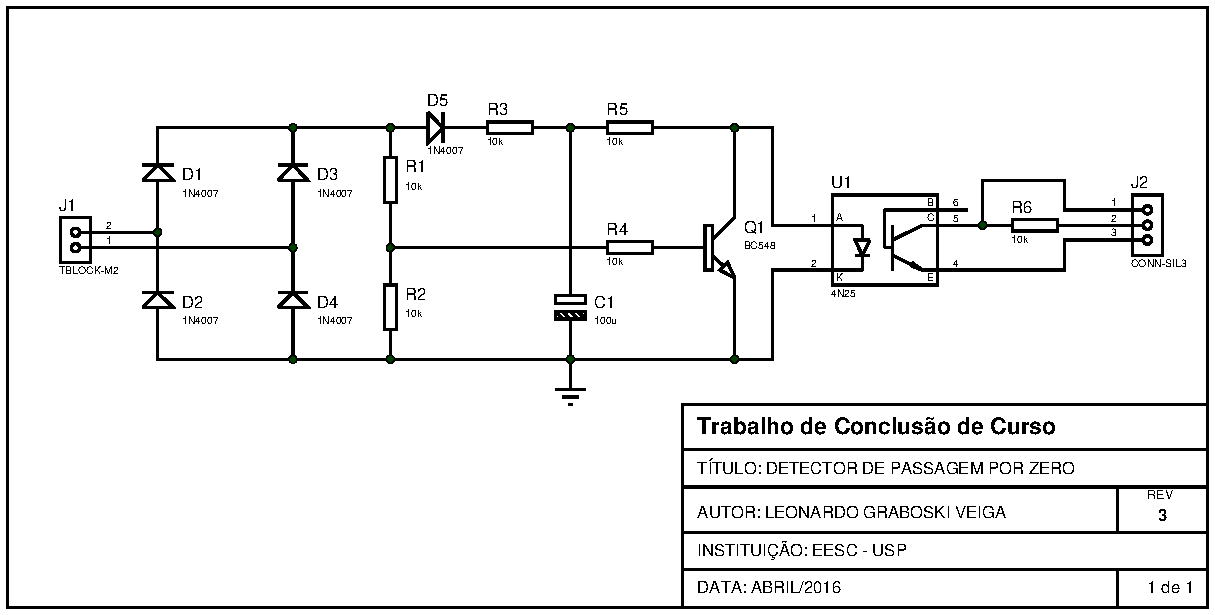
\includegraphics[scale=0.15]{./Resources/proteus/ZeroCrossing.png}
	\captionsetup{justification=centering}
	\caption[Circuito detector de passagem por zero da sen�ide da rede]{Circuito detector de passagem por zero da sen�ide da rede}
	\label{zero_sch}
\end{figure}

%\subsection{Detector de n�vel de l�quido}

%\subsection{mais o que?}



%%%%%%%%%%%%%%%%%%%%%%%%%%%%%%%%%%%%%%%%%%%%%%%%%%%%%%%%%%%%%%%%%%%%%%%%%%

%\section{Sistema de controle de temperatura}
%\subsection{Resistores de aquecimento}

\subsection{Controlador PID}

